Many weather forecasting, assimilation, and dissemination systems are developed to reduce the damage causing by natural disasters such as floods, storms, hurricanes, and even droughts.
Other countries are also using those systems while adopting them to specific weather conditions.
This chapter presents a literature review on existing systems and their architectural approaches and designs. In \cref{se:fews}, we present \acrfull{fews}, an open model integration framework. \acrfull{lead}, an open data handling platform distributed as closed-source software, is presented in \cref{se:lead}.
In \cref{se:dias}, we discuss \acrfull{dias} which is a common data platform that can manage weather data. \acrfull{madis} is another widely used data integration system, which also provides data access with quality controls is presented in \cref{se:madis}. Under each system, we explore their system architecture, scalability, and flexibility.


%%%%%%%%%%%%%%%%%%%%%%%%%%%%%%%%%%%%%%%%%%%%%%%%%%%%%%%%%%%%%%%%%%%%%%%%%%%%%%%%
\section{\acrshort{fews} flow forecasting system}
\label{se:fews}

\acrshort{fews} \cite{Werner2013TheSystem} is developed by Deltares in the Netherland with target audiences/customers of operational forecasting agencies. The \acrshort{fews} codebase is not fully open source at the moment.
Most of models are using a model-centric approach such as inputs, need to be in the format of specific to the model. Also, the outputs produced by the model are specific to the model and hard to utilize by other systems (e.g., FLO2D create human readable text output files). As \acrshort{fews} uses a modular approach it is easier to integrate new models. 
Thus, \acrshort{fews} can be considered as an integration framework or a middleware for the models.

Forecasting processes is creation of modeling steps with combining data transformation algorithms. In the flow, each step process and feed data into the next step. The \acrshort{fews} is flexible enough to integrate new models and algorithms into the core codebase that can use to create new workflows \cite{Werner2013TheSystem}. \acrshort{fews} does not have any inbuilt hydrological modeling capabilities within its codebase. Rather it is a framework that can use to integrate into the system and create workflows for forecasting.

Are proposed by Haggett \cite{Haggett1998AnWales} key elements of a forecasting system are defined as detection, forecasting, then dissemination and warning, and response to the events. The \acrshort{fews} focuses on the forecasting step out from above steps. The main objective of this step is to provide additional lead time by forecasting future hydro-meteorological conditions \cite{Werner2005FloodCatchments}. It is a valid argument that providing accurate predictions with greater lead time can reduce the level of destruction. To forecast, the system should be capable of integrating real-time data from meteorological and hydrological observation network systems, and the disseminate the forecasted results through relevant products to the warning process.

\cref{fi:fews_schematic} shows the connection between the forecasting system to real-time data integration systems and dissemination systems. One of the widely used use cases is to use meteorological forecast data to estimate precipitation, and then use a hydrological and hydraulic model chain to predict the surface water level affects. The hydrological and hydraulic model should be design based on the geographical data. The ground should be analyzed geographically and divide into the catchments. Based on the affected catchment, it can be further divided into sub-catchments to reduce the complexity of the simulation task. Ideally, the forecasting system should be flexible enough to allow modification of models and data, while keeping the most constant way possible of working with forecasters.

\begin{figure}[htp]
    \centering
    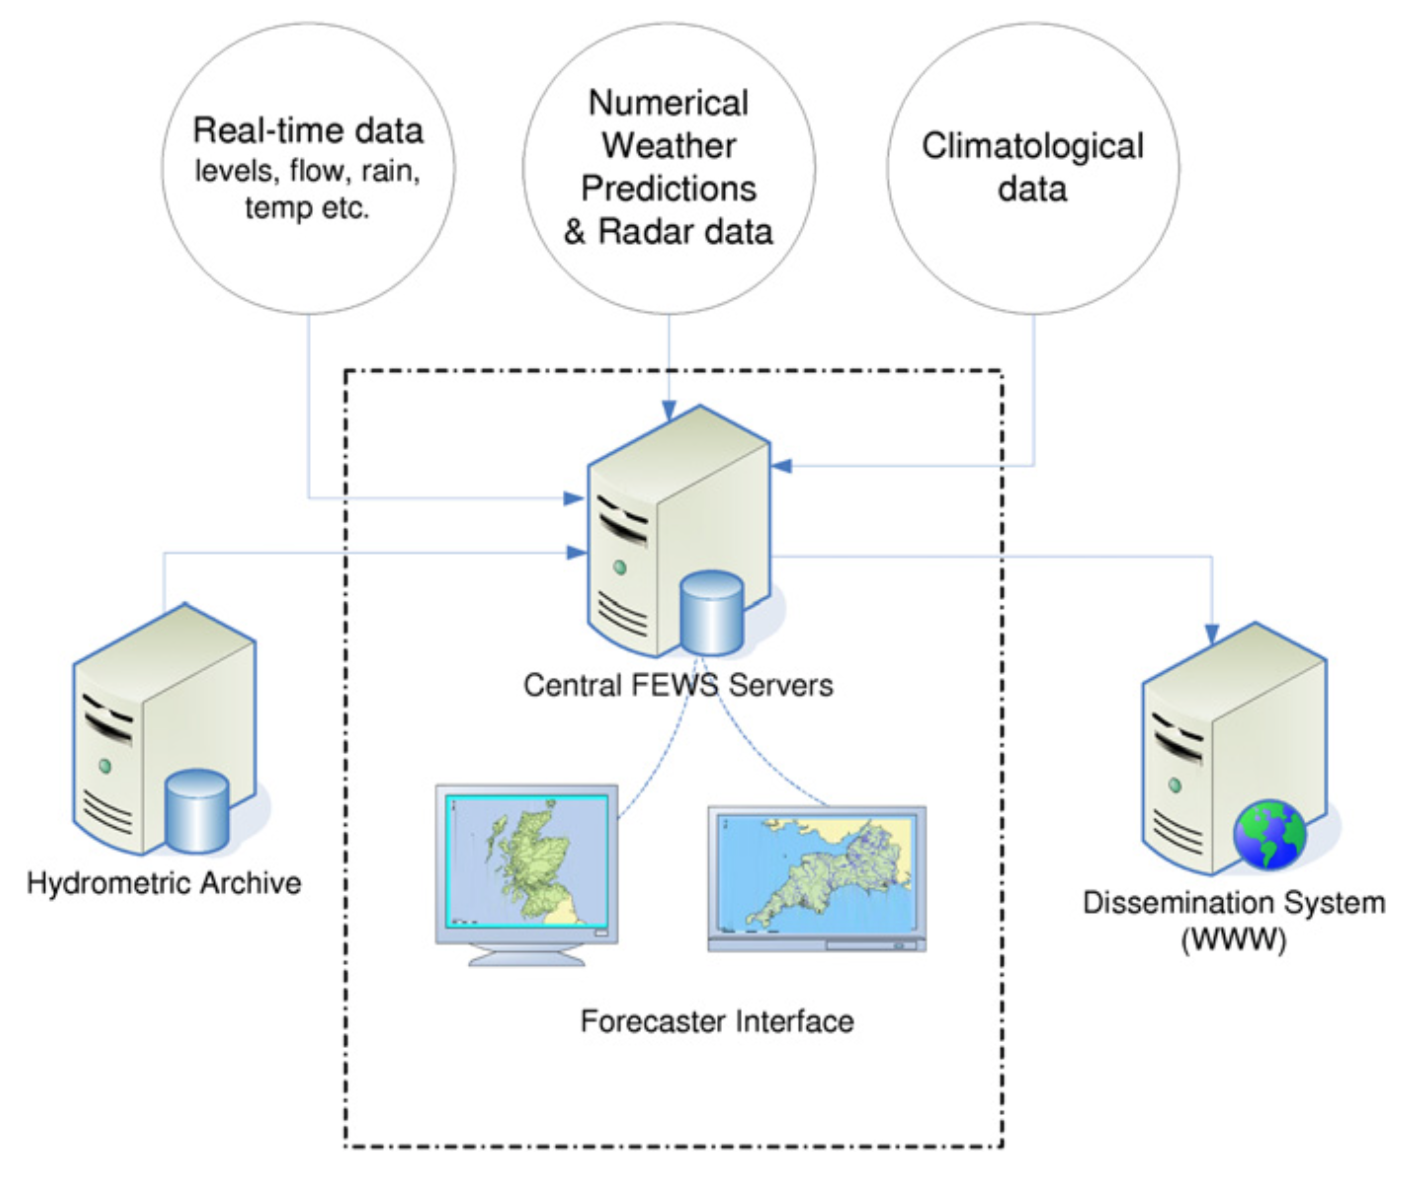
\includegraphics[width=0.7\textwidth]{lit/fews/Schematic-structure-of-a-fl-ood-forecasting-system-showing-the-position-of-Delft-FEWS_W640.png}
    \caption[Schematic structure of a flood forecasting system including \acrshort{fews} and communication among other operational systems]{Schematic structure of a flood forecasting system including \acrshort{fews} and communication among other operational systems \cite{Werner2013TheSystem}.}
    \label{fi:fews_schematic}
\end{figure}

The \acrshort{fews} follows a data-centric approach, with providing a common data-model to interact from all other components. All the timeseries data types are stored in a database which follows a common data model. New models are integrate to the system via using a one of the interfaces provided to interact with the common data-model \cite{Werner2013TheSystem}. As mention in the paper, having a common data-model make easy to store data efficiently. Operations like reporting and sharing the data also make it easy by integrating models. But the problem with this approach is, handling the multiple data formats. \acrshort{fews} overcome this issue by introducing adapters for most of the commonly used data formats. This is a good feature that enables users to easily import data into the system. But at the same time, it's adding additional complexity to the system.

The timeseries data is one of scalar, vector, or grid data, and all of different types are uniformly stored as binary objects in a time series table inside the \acrshort{fews}. Functional compenents or any integrated models do not have direct access to the timeseries table which mentioned above, and those should use the data access module to access the data \cite{Werner2013TheSystem}. As explained in the system interpretation, every time all the data access needs to go through the data access module which causing adding more cost in data access. Since it is storing the different data types as binary objects, there is a penalty in converting data into binary objects and vice versa. Storing all the data in a timeseries table causing all the requests to come into a single data model in a database. Even it gives the advantage of accessing all the data in one place. Since screaming big amount of data is causing a heavy load on the system, causing to slow down in the performance of trying to use the system on a large set of data.

Given above drawback on storing the data in the system, the \acrshort{fews} data model store the timeseries by uniquely identifying based on the location, data type, and source of the data \cite{Werner2013TheSystem}. This allows indexing the database on the above key fields and stores the data separately, to take advantage of putting multiple data resources into the system. As an example, instead of storing the data at a single timeseries table, it is possible to separate and index the database based on the source such as an external source of data or hydrological model of which the timeseries is a result. Or separate by data type and store in multiple storages give the capability for the system to scale with a factor of identical types that can be identified. Example of separation by data types of scalar, vector and gridded will increase the scaling factor by 3x.

Data processing and manipulation is a required process in weather forecasting. 
The data integrated from the external sources are not in the appropriate temporal and spatial format that can directly feed as an input to a forecasting model or use in other application. Therefore, generic data processing steps are a required effort in most model applications in the forecasting environment. Few examples are serial and spatial interpolation, data validation, aggregation and disaggregation, and data fusion \cite{Werner2013TheSystem}. This a vital feature in a forecasting system, and affect the quality and accuracy of the predicted data outputs. Because of the common data model concept in \acrshort{fews}, data processing via these functions is much effective. The system is self-provided some of the generic functions for data processing, but required complex algorithms can be implement as a new Java class via communicate with the \acrfull{api}. It is obvious that for additional feature integration, users should implement the new functional extensions via Java programming language. Users do not have the flexibility of development with some other languages they are familiar with or use the support from another language. As an example, Python language is easy to use for beginners and many data scientists are using this programming language for development and it has many data available libraries for data processing. However, in \acrshort{fews}, users cannot take advantage of such existing tools.

\begin{figure}[htp]
    \centering
    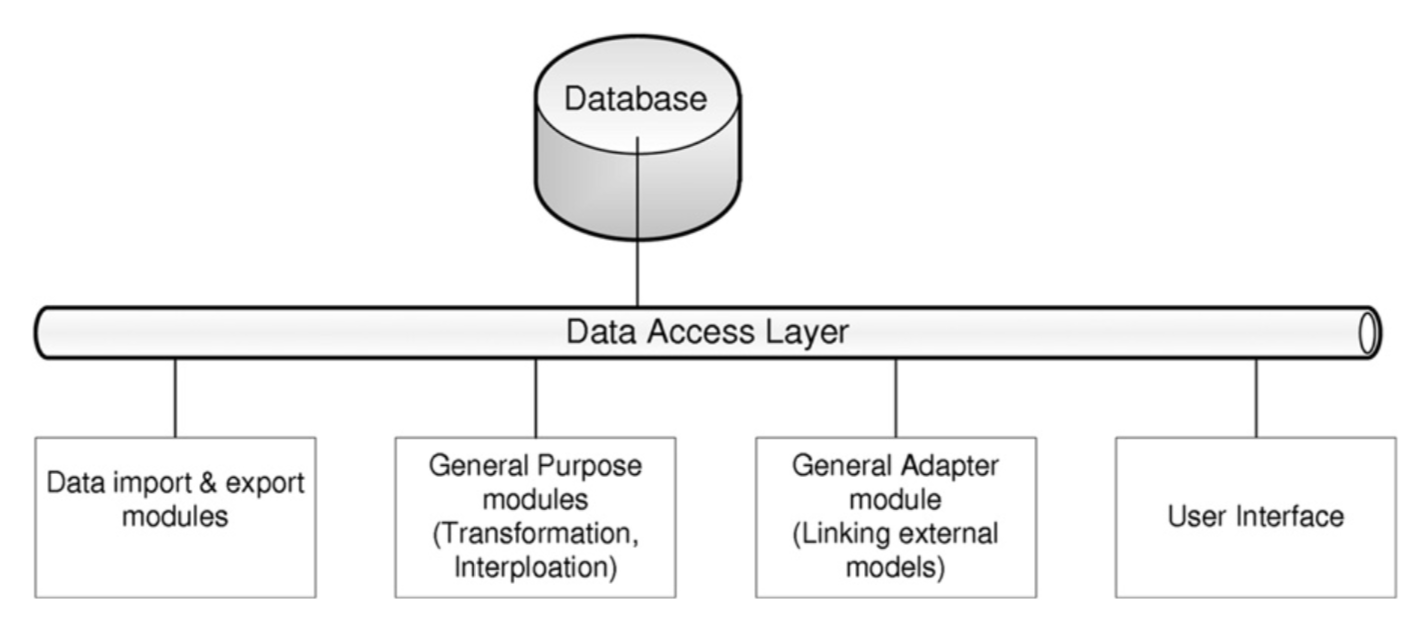
\includegraphics[width=1.0\textwidth]{lit/fews/Architecture-of-Delft-FEWS-showing-the-data-base-the-data-access-layers-and-examples-of_W640.png}
    \caption[Architecture of \acrshort{fews}]{Architecture of \acrshort{fews} \cite{Werner2013TheSystem}.}
    \label{fi:fews_data_layer}
\end{figure}
\db{The \acrshort{fews} supports data processing and modeling library to access scalar and grid timeseries same way}. However, the communicates with the database only via the data access layer as shown in \cref{fi:fews_data_layer} \cite{Werner2013TheSystem}. As it is shown in the figure, it is clearly showing that the system depends on a single database and via the data access layer, all the requests are coming to the database through a connection. It is possible to setup and connect to an enterprise-level database with clustering and shading as a paid solution, to serve many requests as possible. However, the design itself inherently suffers from the database bottleneck which effected by running a large set of timeseries or models.
\dbc{Above highlighted is not clear to me.}
\gkc{Updated}

\begin{figure}[htp]
    \centering
    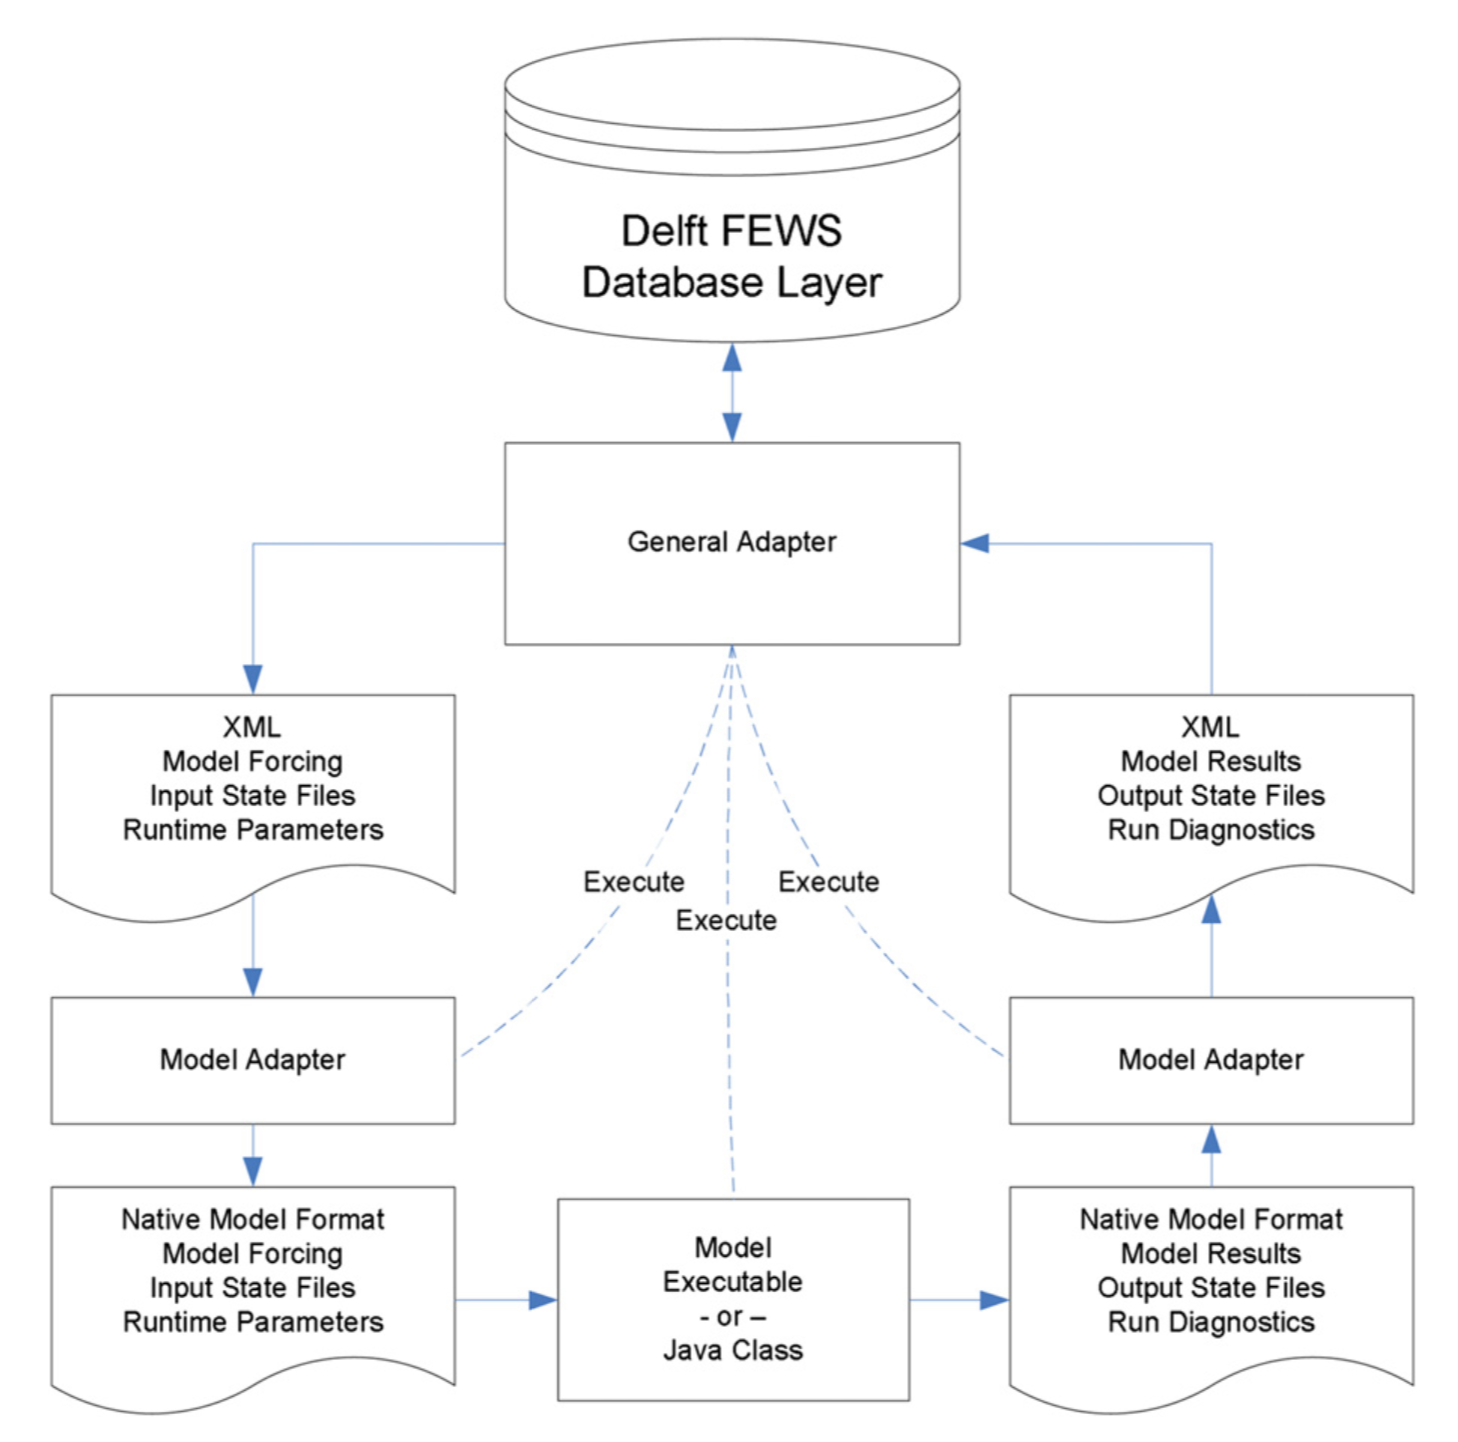
\includegraphics[width=0.8\textwidth]{lit/fews/Linking-Delft-FEWS-with-external-models-The-fi-gure-shows-the-fl-ow-of-data-through-XML_W640.png}
    \caption[\acrshort{fews} integration with external models]{\acrshort{fews} integration with external models \cite{Werner2013TheSystem}.}
    \label{fi:fews_general_adapter}
\end{figure}
One of the simple and most effective features in the \acrshort{fews} is an open approach to the integration of models and data. The concept of the open modeling framework is used by the \acrshort{fews} which is proposed by open model integration \cite{Kokkonen2003InterfacingXML}. It simply gives the flexibility to allow operators to integrate more models as well as variations of the same model and come up with new integration flows as much as possible.
The users need to mentioned the input timeseries via XML configurations, and \acrshort{fews} generates the input data as XML files. Then using an adapter developed for the model transforms the data into required format for the model as a preprocessing step. Next \acrshort{fews} executes the model and model generates the output after successful completion. In the post processing step, the model result data transform to the XML files which can import into the data model as shown in \cref{fi:fews_general_adapter} \cite{Werner2013TheSystem}. The process is simple and consistent throughout all the model integration. The model execute by the \acrshort{fews} or the model adapter which is causing tide coupling into the execution process in the system. Users do not have the flexibility to run the models with different configurations such as running with parallel execution. That may be overcome by triggering an external process at the execution time, but it introduces more difficulty for handling after model executed successfully, preceding to the next step in the process. This part of the system feature is not focused on the \acrshort{wdias} and user has to come up with own flow or use existing scientific flow management system. Yet, it is a concept that needs to be discussed and understand properly to design a data integration and assimilation system. However, the \acrshort{wdias} is capable of integrating workflow mechanism with its extendable architecture.

Data exchange with the model is mainly done via XML files. It is possible to happen, these XML files become very large, which can lead to I/O bottlenecks and causing performance issues \cite{Werner2013TheSystem}. This issue is thoroughly discussed in previous paragraphs and the authors of the \acrshort{fews} \cite{Werner2013TheSystem} seem to be noticed and accept it here. For overcoming this issue they introduced the file-based exchange of data. This includes the use of binary XML files, the streaming of files via memory and the use of \acrshort{netCDF} files. But far as for the users, it seems to be adding more complexity and context to get higher performance via the system.

The \acrshort{fews} provides a list of adapter available. If an adapter is not available for a given model, the user has to implement the adapter for the model and \acrshort{fews} has the flexibility creating a new adapter. But the effort that required to develop an adapter for a model will vary depending on the complexity of the model required data formats \cite{Werner2013TheSystem}. If the users want to use an existing adapter and need to configure something not supported via the existing adapter, it is hard to get done. Also, there are some cases it is hard to develop an adapter or running alongside the \acrshort{fews}. As an example, the FLO2D model is using for hydrologic modeling and the model only supports only on Windows based operating systems. If you setup the system on Linux based operating system and using Linux based models, it is hard for users to come up with a solution for integrating the FLO2D models.
The \acrshort{fews} support creating workflow process and allow users to run multiple models parallel or run those sequentially as needed, but the scope of the \acrshort{wdias} is not focused on adding such a feature in the system, rather user has to use a scientific workflow management system or come up with own version of workflow.
